%%%%%%%%%%%%%%%%%%%%%%%%%%%%%%%%%%%%%%%%%%%%%%%%%%%%%%%%%%%%%%%%%%%%
%%%%%%%%%%%%%%%%%%%%%%%%%%%%%%%%%%%%%%%%%%%%%%%%%%%%%%%%%%%%%%%%%%%%
%%                                                                %%
%% Esimerkki opinnäytteen tekemisestä LaTeX:lla 20130926          %%
%% Alkuperäinen versio Luis Costa,  muutokset Perttu Puska        %%
%%                                                                %%
%% Tähän esimerkkiin kuuluu tiedostot                             %%
%%               opinnaytepohja.tex (versio 1.7)                  %%
%%               aaltothesis.sty (versio 1.7)                     %%
%%               kuva1.eps                                        %%
%%               kuva2.eps                                        %%
%%                                                                %%
%%                                                                %%
%% Kääntäminen                                                    %%
%% latex:                                                         %%
%%             $ latex opinnaytepohja                             %%
%%             $ latex opinnaytepohja                             %%
%%                                                                %%
%%   Tuloksena on tiedosto opinnayte.dvi, joka                    %%
%%   muutetaan ps-muotoon seuraavasti                             %%
%%                                                                %%
%%             $ dvips opinnaytepohja -o                          %%
%%                                                                %%
%% Selittävät kommentit on tässä esimerkissä varustettu           %%
%% %%-merkeillä ja muutokset, joita käyttäjä voi tehdä,           %%
%% on varustettu %-merkeillä                                      %%
%%                                                                %%
%%%%%%%%%%%%%%%%%%%%%%%%%%%%%%%%%%%%%%%%%%%%%%%%%%%%%%%%%%%%%%%%%%%%
%%%%%%%%%%%%%%%%%%%%%%%%%%%%%%%%%%%%%%%%%%%%%%%%%%%%%%%%%%%%%%%%%%%%

%% Käytä toinen näistä, jos kirjoitat suomeksi:
%% ensimmäinen, jos käytät pdflatexia (kuvat on oltava pdf-tiedostoina)
%% toinen, jos haluat tuottaa ps-tiedostoa (käytä eps-formaattia kuville).
%%
%% Use one of these you write in Finnish:
%% the 1st when using pdflatex (use pdf figures) or
%% the 2nd when producing a ps file (use eps figures).
\documentclass[finnish,12pt,a4paper,pdftex]{article}
%\documentclass[finnish,12pt,a4paper,dvips]{article}





%% Käytä näitä, jos kirjoitat englanniksi
%%
%% Uncomment one of these if you write in English
%\documentclass[english,12pt,a4paper,pdftex]{article}
%\documentclass[english,12pt,a4paper,dvips]{article}

%% Tämä paketti on pakollinen
%% Valitse korkeakoulusi näistä: arts, biz, chem, elec, eng, sci.
%% Valiste editorisi käyttämä merkkikoodaustapa: utf8, latin1
%%
%% This package is required
%% Choose your school from arts, biz, chem, elec, eng, sci.
%% Choose the character encoding scheme used by your editor: utf8, latin1
\usepackage[elec,utf8]{aaltothesis} % 
%\usepackage[elec,latin1]{aaltothesis}

%% Jos käytät latex-komentoa käännettäessä (oletusarvo), 
%% kuvat kannattaa tehdä eps-muotoon. Älä käytä ps-muotoisia kuvia!
%% Käytä seuraavaa latex-komennon ja eps-kuvien kanssa 
%%
%% Jos taas käytät pdflatex-komentoa, joka kääntää tekstin suoraan
%% pdf-tiedostoksi, kuvasi on oltava jpg-formaatissa tai pdf-formaatissa.
%%
%% Use this if you run pdflatex and use jpg/pdf-format pictures.
%%
\usepackage{graphicx}
\usepackage{float}

%% Jos et jostain syystä pidä, miten alla oleva hyperref-paketti käyttää
%% fontteja, värejä yms., käytä tämän paketin makroja muuttamaan
%% fonttimäärittelyt. Katso paketin dokumentaatiota. Paketti määrittelee
%% \url-makron, joten ota paketti käyttöön, jos et käytä hyperref-pakettia.
%%
%% Use the macros in this package to change how the hyperref package below 
%% typesets its hypertext -- hyperlink colour, font, etc. See the package
%% documentation. It also defines the \url macro, so use the package when 
%% not using the hyperref package.
%\usepackage{url}

%% Saat pdf-tiedoston viittaukset ja linkit kuntoon seuraavalla paketilla.
%% Paketti toimii erityisen hyvin pdflatexin kanssa. 
%%
%% Use this if you want to get links and nice output with pdflatex
\usepackage[pdfpagemode=None,colorlinks=true,urlcolor=red,%
linkcolor=blue,citecolor=black,pdfstartview=FitH]{hyperref}

%% Matematiikan fontteja, symboleja ja muotoiluja lisää, näitä tarvitaan usein 
%%
%% Use this if you write hard core mathematics, these are usually needed
\usepackage{amsfonts,amssymb,amsbsy}  


%% Vaakasuunnan mitat, ÄLÄ KOSKE!
\setlength{\hoffset}{-1in}
\setlength{\oddsidemargin}{35mm}
\setlength{\evensidemargin}{25mm}
\setlength{\textwidth}{15cm}
%% Pystysuunnan mitat, ÄLÄ KOSKE!
\setlength{\voffset}{-1in}
\setlength{\headsep}{7mm}
\setlength{\headheight}{1em}
\setlength{\topmargin}{25mm-\headheight-\headsep}
\setlength{\textheight}{23cm}

\usepackage{setspace}  % KYPSYYSNÄYTETTÄ VARTEN


%% Kaikki mikä paperille tulostuu, on tämän jälkeen
%%
%% Output starts here
\begin{document}

%% Korjaa vastaamaan korkeakouluasi, jos automaattisesti asetettu nimi on 
%% virheellinen 
%%
%% Change the school field to describe your school if the autimatically 
%% set name is wrong
% \university{aalto University}{aalto-Yliopisto}
% \school{School of Electrical Engineering}{SähköTekniikan korkeakoulu}

%% Vain kandityölle: Korjaa seuraavat vastaamaan koulutusohjelmaasi
%%
%% Only for B.Sc. thesis: Choose your degree programme. 
\degreeprogram{Automation and Systems Technology}%
{Automaatio- ja systeemitekniikka}
%%

%% Vain DI/M.Sc.- ja lisensiaatintyölle: valitse laitos, 
%% professuuri ja sen professuurikoodi. 
%%
%% Only for M.Sc. and Licentiate thesis: Choose your department,
%% professorship and professorship code. 
\department{Department of Automation and Systems Technology}%
{Automaatio- ja systeemitekniikan laitos}
\professorship{Systems Technology}{Systeemitekniikka}
\code{AS-74}
%%

%% Valitse yksi näistä kolmesta
%%
%% Choose one of these:
\univdegree{BSc}
%\univdegree{MSc}
%\univdegree{Lic}

%% Oma nimi
%%
%% Should be self explanatory...
\author{Juho Salmi}

%% Opinnäytteen otsikko tulee vain tähän. Älä tavuta otsikkoa ja
%% vältä liian pitkää otsikkotekstiä. Jos latex ryhmittelee otsikon
%% huonosti, voit joutua pakottamaan rivinvaihdon \\ kontrollimerkillä.
%% Muista että otsikkoja ei tavuteta! 
%% Jos otsikossa on ja-sana, se ei jää rivin viimeiseksi sanaksi 
%% vaan aloittaa uuden rivin.
%% 
%% Your thesis title. If the title is very long and the latex 
%% does unsatisfactory job of breaking the lines, you will have to
%% break the lines yourself with \\ control character. 
%% Do not hyphenate titles.
\thesistitle{Modeling and Simulating Climate Change with System Dynamics}{Ilmastonmuutoksen systeemidynaaminen mallinnus ja simulointi}

\place{Espoo}
%% Kandidaatintyön päivämäärä on sen esityspäivämäärä! 
%% 
%% For B.Sc. thesis use the date when you present your thesis. 
\date{5.10.2013}

%% Kandidaattiseminaarin vastuuopettaja tai diplomityön valvoja.
%% Huomaa tittelissä "\" -merkki pisteen jälkeen, 
%% ennen välilyöntiä ja seuraavaa merkkijonoa. 
%% Näin tehdään, koska kyseessä ei ole lauseen loppu, jonka jälkeen tulee 
%% hieman pidempi väli vaan halutaan tavallinen väli.
%%
%% B.Sc. or M.Sc. thesis supervisor 
%% Note the "\" after the comma. This forces the following space to be 
%% a normal interword space, not the space that starts a new sentence. 
\supervisor{D.Sc.\ (Tech.) Pekka Forsman}{TkT Pekka Forsman}

%% Kandidaatintyön ohjaaja(t) tai diplomityön ohjaaja(t)
%% 
%% B.Sc. or M.Sc. thesis advisors(s). 
%%
%% Note that there has been a change in the official EN translation
%% of the Finnish title ``ohjaaja'' which in the previous version (1.5) 
%% of this document was called ``instructor''. The recommended
%% translation is now ``advisor''.  
%% However, the LaTeX internal variable remains \instructor
%% as there is little point to change the variable name. 
%%
%\instructor{Prof. Pirjo Professori}{Prof. Pirjo Professori}
%\instructor{D.Sc.\ (Tech.) Olli Ohjaaja}{TkT Olli Ohjaaja}
\instructor{M.Sc.\ (Tech.) Tomi Sorasalmi}{DI Tomi Sorasalmi}
\instructor{D.Sc.\ (Tech.) Pekka Forsman}{TkT Pekka Forsman}

%% Aaltologo: syntaksi:
%% \uselogo{aaltoRed|aaltoBlue|aaltoYellow|aaltoGray|aaltoGrayScale}{?|!|''}
%% Logon kieli on sama kuin dokumentin kieli
%%
%% Aalto logo: syntax:
% \uselogo{aaltoRed|aaltoBlue|aaltoYellow|aaltoGray|aaltoGrayScale}{?|!|''}
%% Logo language is set to be the same as the document language.
\uselogo{aaltoRed}{''}

%% Tehdään kansilehti
%%
%% Create the coverpage
\makecoverpage


%% Suomenkielinen tiivistelmä
%% 
%% Finnish abstract
%%
%% Tiivistelmän avainsanat
\keywords{Systeemidynamiikka, ilmastonmuutos}
%% Tiivistelmän tekstiosa
\begin{abstractpage}[finnish]
Placeholderina alkuperäinen tehtävänanto: Systeemidynamiikkaa on käytetty paljon ympäristöongelmien sekä ilmastonmuutoksen mallintamisessa. Kandityön tarkoituksena on tehdä kirjallisuustarkastelu ilmastonmuutoksen mallintamisessa käytetyistä systeemidynaamisista malleista, eri lähestymistavoista, eri resoluution malleista ja sovellusalueista. Pyritäänkö malleilla ymmärtämään ilmastonmuutosta paremmin vai kommunikoimaan jo tiedossa olevia ongelmia. Käyttävätkö vain päättäjät malleja vai onko kehitetty suurelle yleisölle tarkoitettuja malleja/pelejä. Mitä uutta systeemidynaaminen mallintaminen on tuonut ilmastonmuutoksen mallintamiseen.
\end{abstractpage}

%% Pakotetaan uusi sivu varmuuden vuoksi, jotta 
%% mahdollinen suomenkielinen ja englanninkielinen tiivistelmä
%% eivät tule vahingossakaan samalle sivulle
%%
%% Force new page so that English abstract starts from a new page
\newpage
%
%% English abstract, uncomment if you need one. 
%% 
%% Abstract keywords
\keywords{System dynamics, climate change}
%% Abstract text
\begin{abstractpage}[english]
 Abstract in English. 
\end{abstractpage}
%% Note that 
%% if you are writting your master's thesis in English place the English
%% abstract first followed by the possible Finnish abstract

%% Esipuhe 
%%
%% Preface
\mysection{Esipuhe}
%\mysection{Preface}




\vspace{5cm}
Otaniemi, 24.9.2013

\vspace{5mm}
{\hfill Juho T.\ Salmi \hspace{1cm}}

%% Pakotetaan varmuuden vuoksi esipuheen jälkeinen osa
%% alkamaan uudelta sivulta
%%
%% Force new page after preface
\newpage


%% Sisällysluettelo
%% 
%% Table of contents. 
\thesistableofcontents

% TÄNNE VOISI LISÄTÄ TERMISTÖN: FI - ENG

%% Symbolit ja lyhenteet
%%
%% Symbols and abbreviations
%\mysection{Symbolit ja lyhenteet}
%\mysection{Symbols and abbreviations}
%\subsection*{Symbolit}
%%\subsection*{Symbols}
%
%\begin{tabular}{ll}
%%$|a_{ij}|^2$, $|a_i|^2$ & probability of two electrons having momenta
%%    $\boldsymbol p_i$ and $\boldsymbol p_j$ ($\boldsymbol p_i$ for $|a_i|^2$) \\
%%                 & at any given instant \\
%$\mathbf{B}$  & magneettivuon tiheys  \\
%$c$              & valon nopeus tyhjössä $\approx 3\times10^8$ [m/s]\\
%%$p$              & magnitude of momentum \\
%%$\boldsymbol p$, $\boldsymbol p_i$, $\boldsymbol p_i^{'}$  & momentum vector \\
%%$p$              & magnitude of momentum \\
%%$\boldsymbol p$, $\boldsymbol p_i$, $\boldsymbol p_i^{'}$  & momentum vector \\
%%$\boldsymbol P$  &  \\
%%$p_{\mathrm{F}}$ & Fermi momentum \\
%$\omega_{\mathrm{D}}$    & Debye-taajuus \\
%%$\omega_{\mathrm{latt}}$ & hilan keskimääräinen fononitaajuus \\
%$\uparrow$       & elektronin spinin suunta ylöspäin\\
%%$\downarrow$     & elektronin spinin suunta alaspäin
%\end{tabular}
%
%\subsection*{Operaattorit}
%%\subsection*{Opetators}
%
%\begin{tabular}{ll}
%$\nabla \times \mathbf{A}$              & vektorin $\mathbf{A}$ roottori\\
%$\displaystyle\frac{\mbox{d}}{\mbox{d} t}$ & derivaatta muuttujan $t$ suhteen\\
%[3mm]
%$\displaystyle\frac{\partial}{\partial t}$  & osittaisderivaatta muuttujan $t$ suhteen \\[3mm]
%$\sum_i $                       & Summa indeksin $i$ yli\\
%$\mathbf{A} \cdot \mathbf{B}$    & vektorien $\mathbf{A}$ ja $\mathbf{B}$ pistetulo
%\end{tabular}

\begin{onehalfspacing} % KYPSYYSNÄYTETTÄ VARTEN

%\subsection*{Lyhenteet}
%\subsection*{Abbreviations}

%\begin{tabular}{ll}
%SD         & systeemidynamiikka \\
%\end{tabular}


%% Sivulaskurin viilausta opinnäytteen vaatimusten mukaan:
%% Aloitetaan sivunumerointi arabialaisilla numeroilla (ja jätetään
%% leipätekstin ensimmäinen sivu tyhjäksi, 
%% ks. alla \thispagestyle{empty}).
%% Pakotetaan lisäksi ensimmäinen varsinainen tekstisivu alkamaan 
%% uudelta sivulta clearpage-komennolla. 
%% clearpage on melkein samanlainen kuin newpage, mutta 
%% flushaa myös LaTeX:n floatit 
%% 
%% Corrects the page numbering, there is no need to change these
\cleardoublepage
\storeinipagenumber
\pagenumbering{arabic}
\setcounter{page}{1}



%% Leipäteksti alkaa
%%
%% Text body begins. Note that since the text body
%% is mostly in Finnish the majority of comments are
%% also in Finnish after this point. There is no point in explaining
%% Finnish-language specific thesis conventions in English.
\section{Johdanto}
%\section{Introduction}

%% Ensimmäinen sivu tyhjäksi
%% 
%% Leave first page empty
\thispagestyle{empty}

Ihmiselle on luontaista ajatella, että asioille on selkeät ja suoraviivaiset syy-seuraus-suhteet: yksi asia vaikuttaa toiseen. Maailma ei kuitenkaan olen niin yksinkertainen ja lineaarinen, vaan asiat ovat mitä moninaisimmin tavoin vuorovaikutuksessa toistensa kanssa. Systeemidynamiikka on tapa ymmärtää, mallintaa ja simuloida tätä vuorovaikutusta sekä niiden muodostamaa monimutkaista systeemiä. 

% Tähän voisi olla mielenkiintoista laittaa vertailu lineaarisesta tavasta ajatella sekä systeemidynaamisesta tavasta ajatella. Etenkin jos löytyisi naseva vertaus ilmastonmuutoksen puolelta. 

Systeemidynaaminen malli rakentuu varantojen, virtausten sekä takaisinkytkettyjen silmukoiden varaan. Systeemidynamiikan tapa lähestyä asioita tarjoaa erinomaiset työkalut päätöksenteolle ja ajattelulle yleisesti. Yksi keskeinen systeemidynamiikan etu on sen ilmaisuvoima. Kausaalidiagrammit kiteyttävät hyvin, mistä systeemidynaamisessa mallissa on kyse. Lisäksi systeemidynaamisia malleja on verrattaen luonteva lähteä rakentamaan tunnettujen ja tutkittujen kausaliteettien varaan. Systeemidynaamiset mallit ovat myös laskennallisesti kevyitä, joten mallin parametrien muuttamisen vaikutusten demonstroiminen käy hetkessä.  

Ilmastonmuutos on tilastollisesti merkittävää ja pitkäkestoista muutosta globaalissa tai paikallisessa ilmastossa. Tässä kandidaatintyössä keskitytään ihmisen toiminnasta johtuvaan globaaliin ilmastonmuutokseen, erityisesti ilmaston lämpenemiseen. 

Ilmastonmuutosta mallinnetaan, jotta kykenisimme arvioimaan, millaisia vaikutuksia toiminnallamme on, ja millaisin päätöksin voisimme saada ilmaston kehittymään haluttuun suuntaan. Ilmastoa ja sen muutosta mallinnetaan tieteellisiin tarkoituksiin pääasiassa tarkoilla fysikaalisilla malleilla. Tarkat mallit ovat laskennallisesti raskaita, eivätkä ne ole maallikon tai poliittisen päättäjän ymmärrettävissä. Systeemidynamiikalla voidaan ilmastomalli esittää ymmärrettävässä muodossa siten, että päättäjä kykeneei hahmottamaan, mistä mallissa on kyse. Tämän lisäksi systeemidynaaminen simulaatio on ajettavissa hetkessä, joten esimerkiksi ympäristöpoliittisten päätösten seuraukset on nopeasti havainnollistettavissa. 

Tämän kandidaatintyön tavoite on tutkia systeemidynamiikkaa ja sen soveltamista ilmastonmuutoksen mallintamiseen ja simulointiin. Luvussa \ref{sysdyn} otetaan katsaus systeemidynamiikan perusperiaatteisiin. Luvussa \ref{ilmasto} tutustutaan ilmastonmuutokseen ja sen mallintamiseen. Ilmastonmuutoksen systeemidynaaminen mallintaminen havainnollistetaan kahta esimerkkiä käyttäen. Lopuksi luvussa \ref{yhteenveto} tehdään yhteenveto tämän kandidaatintyön löydöksistä ja havainnoista. 


%% Opinnäytteessä jokainen osa alkaa uudelta sivulta, joten \clearpage
%%
%% In a thesis, every section starts a new page, hence \clearpage
\clearpage

% \section{Teoreettinen tausta}
% \section{Background}


\section{Systeemidynamiikka \label{sysdyn}}


Systeemi eli järjestelmä tarkoittaa toistensa kanssa vuorovaikutuksessa olevien osien muodostamaa kokonaisuutta \cite{Flood1988}. Systeemidynamiikka on tietokoneavusteinen lähestymistapa päätöksentekoon ja mutkikkaiden systeemien mallintamiseen \cite{WhatIsSystemDynamics}. Mutkikkaalle systeemille ei ole yksikäsitteistä määritelmää \cite{Zadeh1973}, mutta systeemidynamiikalla kyetään mallintamaan erityisesti systeemien takaisinkytkentöjä ja epälineaarisuuksia \cite{WhatIsSystemDynamics}, jotka ovat systeemin mutkikkuutta lisääviä ominaisuuksia \cite{Zadeh1973}. % Perustele termin valinta?

Tämän luvun tavoite on tutustuttaa lukija systeemidynamiikan perusperiaatteisiin, jotka ovat välttämättömiä luvun \ref{ilmasto} systeemidynaamisten ilmastomallien ymmärtämiseksi. Alaluvussa \ref{sysdyn:historia} selvitetään, miksi ja miten systeemidynamiikka syntyi ja kehittyi, alaluvussa \ref{sysdyn:paatos} tutustutaan systeemiajatteluun ja päätöksentekoon, alaluvussa \ref{sysdyn:takaisinkytkenta} systeemien takaisinkytkentöihin sekä alaluvussa \ref{sysdyn:vvv} systeemien viiveisiin, varastoihin ja virtauksiin. 

\subsection{Systeemidynamiikan historia \label{sysdyn:historia}} 

% Systeemidynamiikan ymmärtämiseen auttaa sen historian tunteminen. Tämä alaluku käsittelee systeemidynamiikan historiaa, etenkin sen syntyyn ja kehitykseen vaikuttaneita tekijöitä. 

Systeemidynamiikan on alunperin perustanut Jay W. Forrester, joka vuonna 1956 siirtyi MIT:ssä sähkötekniikan alalta Sloan School of Managementiin tekemään operaatiotutkimusta. Forrester alkoi tutkia, miksi General Electricin tehtailla työskenneltiin välillä kolmessa vuorossa ja välillä jouduttiin puolet työntekijöistä irtisanomaan. Forrester alkoi yhdistellä säätö- ja systeemiteoriaa operaatiotutkimukseen ja ryhtyi simuloimaan teollisuustuotantoa sekä luomaan sille säätöjärjestelmiä tietokoneavusteisesti. Tämän tutkimuksen pohjalta syntyi systeemidynamiikka ja alan ensimmäinen julkaisu Industrial Dynamics \cite{Forrester1961}. \cite{Forrester1989} 

Forresterin \cite[s. 398--399]{Forrester1968} mukaan sen aikainen operaatiotutkimus ei tarjonnut hyviä työkaluja laajoihin, ylimmän tason johtamisen haasteisiin. Operaatiotutkimuksessa keskityttiin pääsääntöisesti yksittäisten, irrallisten päätösten seurausten hahmottelemiseen oletuksella, että päätöksen seuraukset eivät vaikuta päätöksentekoon vaikuttaviin tekijöihin. Oletusta kutsutaan avoimen silmukan oletukseksi. Tällaisella tarkastelulla pystyttiin yksinkeraistamaan analyysiä, mutta näin kyettiin tarkastelemaan riittävällä tarkkuudella vain yksinkertaisia, lineaarisia tilanteita, siinä missä systeemidynamiikalla pystytään ottamaan huomioon mutkikkaidenkin järjestelmän osien takaisinkytkennät ja epälineaarisuudet. Takaisinkytkettyjä systeemeitä oli jo pitkään tutkittu ja hyödynnetty insinööritieteissä, biologiassa ja taloustieteessä, mutta niitä oli vasta hiljattain alettu ymmärtää. 

Samat takaisinkytkettyjen systeemien periaatteet olivat yleistettävissä eri tieteenaloille, minkä johdosta monilla aloille otettiin systeemidynaamisia menetelmiä käyttöön. Systeemidynamiikasta kehittyikin nopeasti hyvin poikkitieteellinen ala. \cite{WhatIsSystemDynamics, Forrester1968, Sterman2000} % Tätä voisi hioa



\subsection{Systeemiajattelu ja päätöksenteko \label{sysdyn:paatos}}

Systeemiajattelu on tapa jäsentää maailma mielessään mutkikkaana systeeminä, ja sen työkaluna voi käyttää systeemidynamiikkaa \cite[s. 4--5]{Sterman2000}. Sterman \cite[s. 4--5]{Sterman2000} vertaa systeemidynamista mallintamista lentosimulaattoriin: lentosimulaattori opettaa turvallisesti lentäjän lentämään ja systeemidynamiikka johtajan systeemiajattelemaan eli hahmottamaan johtamansa organisaation systeeminä. 

Systeemidynamiikan asiantuntijat käyttävät usein sanontaa: "Tie helvettiin on kivetty hyvillä aikomuksilla." Stermanin \cite[s. 5--6]{Sterman2000} mukaan hyvää tarkoittavilla päätöksillä saatetaan tehdä ongelmia pahemmiksi, sillä monilla päätöksillä on seurauksia, joita on vaikea ennalta arvioida. % Miten tällaiseen sitaattiin viittaa? 

Päätöksenteon maailmankuvan voi jakaa tapahtumasuuntautuneeseen ja takaisinkytkentäsuuntautuneeseen. Seuraava kuva \ref{sysdyn:tapahtumasuuntautunut} esittää tapahtumasuuntautunutta maailmankuvaa. Tapahtumasuuntautuneisuus on ihmiselle luontevaa, sillä se on lineaarista ja suoraviivaista: jokaisella teolla on seurauksensa. Kun on tilanne ja asetetut tavoitteet, niin ongelma syntyy siitä, kun ne poikkeavat toisistaan. Mitä enemmän tilanne ja tavoite poikkeavat toisistaan, sitä suurempi ongelma. Ongelman ratkaisemiseksi tarvitaan päätös, joka johtaa haluttuun lopputulokseen. Päätös voi kuitenkin vaikuttaa ympäröivään tilanteeseen mitä moninaisimmin tavoin. Tapahtumasuuntautuneessa maailmankuvassa tätä ei tyypillisesti huomioida, ja päätöksistä saattaa seurata odottamattomia sivuvaikutuksia. \cite[s. 10]{Sterman2000}

\begin{figure}[H]
\centering 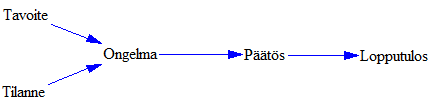
\includegraphics{tapahtuma}
\caption{Tapahtumasuuntautunut maailmankuva. \cite[s. 10]{Sterman2000} \label{sysdyn:tapahtumasuuntautunut}}
\end{figure}

Stermanin \cite[s. 11]{Sterman2000} mukaan sivuvaikutuksia ei ole todellisuudessa kuitenkaan olemassa. On vain olemassa vuorovaikutussuhteita, joita ei ole otettu huomioon. Seuraava kuva \ref{sysdyn:takaisinkytkentasuuntautunut} esittää takaisinkytkentäsuuntautunutta maailmankuvaa. Systeemiajattelijan maailmankuva on takaisinkytkentäsuuntautunut, ja hän ymmärtää päätösten vaikuttavan ympäristön tekijöihin, jotka puolestaan vaikuttavat päätöksiin. 

\begin{figure}[H]
\centering 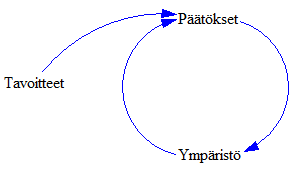
\includegraphics{takaisinkytkentasuuntautunut}
\caption{Takaisinkytkentäsuuntautunut maailmankuva. \cite[s. 11]{Sterman2000} \label{sysdyn:takaisinkytkentasuuntautunut}}
\end{figure}

Maailmankuvaa voi edelleen laajentaa. Seuraava kuva \ref{sysdyn:laajennettutakaisinkytkentasuuntautunut} on laajennettu edellisestä kuvasta \ref{sysdyn:takaisinkytkentasuuntautunut} ottamaan huomioon useampia systeemin tekijöitä. Systeemiajattelija hahmottaa, että päätöksillä on myös muita seurauksia, ja nekin muuttavat ympäristöä. Muuttuva ympäristö vaikuttaa myös tavoitteisiin -- niin omiin kuin muidenkin. Kun ympäristö ja muiden tavoitteet muuttuvat, tekevät muut päätöksiään sen pohjalta, mikä puolestaan muuttaa ympäristöä. \cite[s. 11--12]{Sterman2000}

\begin{figure}[H]
\centering 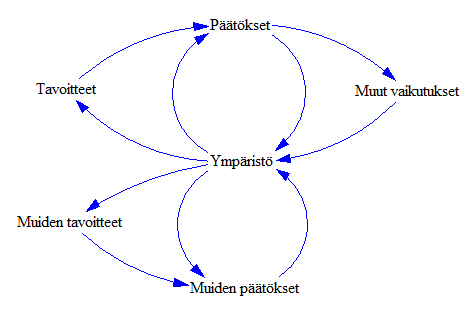
\includegraphics{laajennettutakaisinkytkentasuuntautunut}
\caption{Laajennettu takaisinkytkentäsuuntautunut maailmankuva. \cite[s. 11]{Sterman2000} \label{sysdyn:laajennettutakaisinkytkentasuuntautunut}}
\end{figure}


\subsection{Takaisinkytketyt systeemit \label{sysdyn:takaisinkytkenta}}

Systeemeillä on tuloja ja lähtöjä. Tulot (myös sisääntulo, eng. input) ovat systeemiin tulevia arvoja, jotka vaikuttavat systeemin käyttäytymiseen. Lähdöt (myös ulostulo, eng. output) ovat systeemin käyttäytymisestä seuraavia arvoja. Erilaisilla tuloilla saadaan systeemistä erilaiset lähdöt. Takaisinkytkentä tarkoittaa systeemin lähdön käyttämistä systeemin tulona. Tällöin systeemi kytkeytyy takaisin itseensä, muodostaa kytkennöistä silmukan ja vaikuttaa itse itseensä. Takaisinkytkennästä käytetään erityisesti ihmistieteiden puolella myös termiä "palaute". \cite{Sterman2000, WhatIsSystemDynamics} % Viitteet kuntoon! Perustele termin valinta? 

Stermanin \cite[s. 12]{Sterman2000} mukaan takaisinkytkennät vaikuttavat systeemin mutkikkuuteen enemmän kuin järjestelmän osien mutkikkuus itse. Tämän vuoksi takaisinkytkentöjen löytäminen on keskeisin osa systeemidynaamista mallinnusta. 

Systeemidynaamisia malleja esitetään kausaalidiagrammein, joihin merkitään systeemin osat eli muuttujanimet sekä niiden väliset vuorovaikutussuhteet kausaaliyhteysnuolten avulla. Nuolet piirretään lähtemään muuttujasta, joka vaikuttaa nuolen päätepisteen muuttujaan. Nuoliin merkitään plus- tai miinus merkki sen mukaan, kasvattaako vaiko vähentääkö lähtömuuttujan arvon kasvu tulomuuttujan arvoa. Nuolet piirretään kaareviksi, jotta systeemin dynamiikkaa, etenkin silmukat, olisi helpompi hahmottaa. \cite{Sterman2000}

Takaisinkytkettyjä silmukoita on kahdenlaisia: negatiivisia ja positiivisia. Positiiviset silmukat ovat itseään vahvistavia. Seuraavassa kuvassa \ref{sysdyn:positiivinen} on positiivinen takaisinkytketty silmukka, jossa kanojen määrä lisää munien määrää, mikä puolestaan lisää kanojen määrää. Positiiviset silmukat merkitään kausaalidiagrammiin kuvan \ref{sysdyn:positiivinen} mukaisesti R-kirjaimella, mikä tulee englannin kielen sanasta "reinforcing" eli suomeksi "vahvistava". \cite[s. 12--13]{Sterman2000}\cite{WhatIsSystemDynamics}

\begin{figure}[H]
\centering 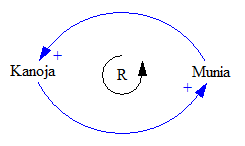
\includegraphics{positiivinen}
\caption{Positiivinen takaisinkytketty silmukka. \cite[s. 13]{Sterman2000} \label{sysdyn:positiivinen}}
\end{figure}

Negatiiviset silmukat ovat itseään tasapainottavia. Seuraavassa kuvassa \ref{sysdyn:negatiivinen} on negatiivinen takaisinkytketty silmukka, jossa kanojen lisääntyminen johtaa siihen, että useampi niistä ylittää tien ja jää auton alle, mikä puolestaan vähentää kanojen määrää, mikä puolestaan vähentää tien ylityksiä. Negatiiviset silmukat merkitään kuvan \ref{sysdyn:negatiivinen} mukaisesti B-kirjaimella, mikä tulee englannin kielen sanasta "balancing" eli suomeksi "tasapainottava". \cite[s. 12--14]{Sterman2000}

\begin{figure}[H]
\centering 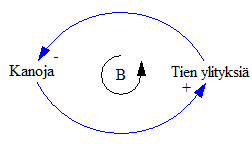
\includegraphics{negatiivinen}
\caption{Negatiivinen takaisinkytketty silmukka. \cite[s. 13]{Sterman2000} \label{sysdyn:negatiivinen}}
\end{figure}

Silmukka on positiivinen, kun siinä on parillinen määrä negatiivisia kytkentöjä. Kuvan \ref{sysdyn:positiivinen} positiivisessa silmukassa on nolla negatiivista kytkentää. Silmukka on negatiivinen, kun siinä on pariton määrä negatiivisia kytkentöjä. Kuvan \ref{sysdyn:negatiivinen} negatiivisessa silmukassa on yksi negatiivinen kytkentä. \cite[s. 12--14]{Sterman2000}

\subsection{Viiveet, varastot ja virtaukset \label{sysdyn:vvv}}

Viiveet aiheuttavat systeemiin hitautta, aiheuttavat värähtelyitä sekä johtavat siihen, että päätösten seuraukset johtavat pitkällä aikajänteellä erilaisiin tilanteisiin kuin lyhyellä aikajänteellä. Seuraavassa kuvassa \ref{sysdyn:viive} on esitetty systeemi, jossa hinnan nousu lisää viiveellä tuotantoa. Kausaalidiagrammeihin viiveet merkitään nuolen päälle joko kahdella poikkiviivalla tai laatikolla, jossa lukee "viive". \cite[s. 150--152]{Sterman2000} 

\begin{figure}[H]
\centering 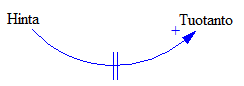
\includegraphics{viive}
\caption{Viiveellinen systeemi \cite[s. 150]{Sterman2000} \label{sysdyn:viive}}
\end{figure}

Varastot ovat systeemin osia, joiden arvo kertyy. Ne tuottavat systeemiin muistia sekä hitautta ja niillä voi kuvata viiveitä. Varastot myös kertovat päättäjille, mikä on systeemin tila. Varastoon voi tulla sisäänvirtauksia ja sieltä voi lähteä ulosvirtauksia. Sisäänvirtaukset kerryttävät ja ulosvirtaukset kuluttavat varaston arvoa. Seuraava kuva \ref{sysdyn:varastovirtaus} on yksinkertainen kausaalidiagrammiesitys varastosta ja virtauksista. Varastot merkitään kausaalidiagrammiin suorakulmioilla, virtauskytkennät virtausnuolilla, virtausmuuttujat venttiilisymboleilla sekä systeemin ulkopuoliset lähteet ja nielut pilvillä. \cite[s. 191--197]{Sterman2000} 

\begin{figure}[H]
\centering 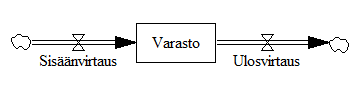
\includegraphics{varastovirtaus}
\caption{Yksinkertainen kausaalidiagrammi varastoista ja virtauksista. \cite[s. 150]{Sterman2000} \label{sysdyn:varastovirtaus}}
\end{figure}

Varaston matemaattinen esitys vastaa integraattoria, joka integroi sisäänvirtauksen ja ulosvirtauksen erotusta alkuhetkestä $t_0$ hetkeen $t$: 

\begin{equation}
  Varasto(t) = \int_{t_0}^t \Big( Sis\ddot{a}\ddot{a}nvirtaus(s) - Ulosvirtaus(s) \Big) ds + Varasto(t_0)
\end{equation} \cite[s. 194--195]{Sterman2000} 

Varastot ja virtaukset ovat intuitiivinen esitystapa, mutta saman dynamiikan voi esittää ilmankin niitä \cite[s. 191--230]{Sterman2000}. Seuraavassa kuvassa \ref{sysdyn:varastovirtauskana} on esitetty kuvan \ref{sysdyn:negatiivinen} negatiivisesti takaisinkytketty silmukka varastojen ja virtausten avulla. Kanojen määrä voidaan ajatella varastona ja tien ylitykset virtauksena, joka vähentää kanojen määrää. Kanojen määrä säätää tien ylitykset -venttiiliä: mitä enemmän kanoja, sitä avonaisempi venttiili ja suurempi virta. 

\begin{figure}[H]
\centering 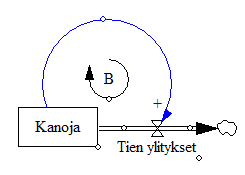
\includegraphics{varastovirtauskana}
\caption{Kuvan \ref{sysdyn:negatiivinen} negatiivisesti takaisinkytketyn silmukan esitys varastojen ja virtausten avulla. \label{sysdyn:varastovirtauskana}}
\end{figure}

% Tänne vielä mahdollisesti kylpyammedynamiikasta juttua sekä muuta systeemidynamiikkasaivartelua, mikä auttaa lukijaa ymmärtämään seuraavat käsitteet

\clearpage
\section{Ilmastonmuutoksen mallintaminen \label{ilmasto}}

Ilmastonmuutoksen mallintamiseen tarvitaan aina jonkinlainen fysikaalinen malli. Raskaimmissa fysikaalisissa malleissa ilmakehä ja meret saatetaan pilkkoa lukuisiksi osiksi neliökilometrin alueisiin ja useisiin kerroksiin. Näiden osien keskinäistä vuorovaikutusta simuloidaan erilaisin kasvihuonekaasujen parametrein. Raskaimpien fysikaalisten mallien simuloimiseen voi supertietokoneeltakin mennä päiväkausia. [viite]

Systeemidynaamiset fysiikkamallit ovat pääsääntöisesti karkeita ja ottavat huomioon vain yksittäisiä maailmanlaajuisia suureita. Näin ollen mallin simuloiminen on nopeaa. Tässä työssä esiteltävien systeemidynaamisten ilmastomallien simuloiminen vie kotikoneella sekunnin murto-osan. Systeemidynaamiset fysiikkamallit viritetään ja validoidaan historiadatalla sekä tarkkojen fysiikkamallien avulla: kun systeemidynaaminen fysiikkamalli tekee oikeita ennustuksia historiadatan pohjalta sekä vastaavia ennustuksia kuin yleisesti hyväksytyt fysiikkamallit, voidaan malli katsoa oikeaksi. [viite]

Fysiikkamallin voi laajentaa ihmisiin. Ilmastomalleilla voidaan myös tutkia, miten ilmastonmuutos vaikuttaa esimerkiksi väestönkasvuun, talouskasvuun ja hyvinvointiin. Tällaisia eri tieteenaloja yhdisteleviä malleja kutsutaan integroiduiksi malleiksi. [viite]

Tämän luvun tavoitteena on tutustuttaa lukija ilmastonmuutoksen mallintamiseen ensin yleisesti ja sitten systeemidynaamisiin malleihin pureutuen. Aluksi alaluvussa \ref{ilmasto:historia} tutustutaan ilmastonmuutoksen ja ilmastomallien historiaan sekä hahmotellaan, miksi myös mallintamiseen on alettu käyttää myös systeemidynaamisia menetelmiä. Seuraavat alaluvut \ref{ilmasto:croads} ja \ref{ilmasto:enroads} esittelevät systeemidynaamiset Climate Interactiven C-ROADS- ja En-ROADS-ilmastomallit. Lopuksi alaluvussa \ref{ilmasto:muut} otetaan lyhyt katsaus muutamaan muuhun tunnettuun ilmastomalliin. 

\subsection{Ilmastomallien historia \label{ilmasto:historia}}

% http://en.wikipedia.org/wiki/History_of_climate_change_science

\subsection{C-ROADS-ilmastomalli \label{ilmasto:croads}}

C-ROADS-ilmastomalli on fysikaalinen ja perustuu Fiddamanin \cite{Fiddaman1997} kehittämään systeemidynaamiseen ilmastomalliin. C-ROADS-ilmastomalli koostuu useasta alimallista. Kullekin kasvihuonekaasulle on oma alimallinsa, samoin metsien kasvattamiselle ja tuhoamiselle, meren pinnan korkeudelle sekä maapallolle kertyneelle lämpöenergialle. \cite{croads}

Kasvihuonekaasuista malliin on otettu hiilidioksidi ($CO_2$), metaani ($CH_4$), typpidioksidi ($N_2O$), perfluorohiiliyhdisteet ($PFC$), rikkiheksafluoridi ($SF_6$) sekä hydrofluorihiiliyhdisteet ($HFC$). Tarkimmin mallissa on esitetty hiilidioksidin kiertokulku, joten kasvihuonekaasuista tässä työssä esitetään vain sen alimalli. 

Seuraava kuva \ref{ilmasto:co2} on yksinkertaistettu hiilidioksidin alimalli, jossa on kuusi varastomuuttujaa, joista kukin kuvaa hiilidioksidivarastoa. Näitä varastoja ovat: ilmakehä (C in Atmosphere), biomassa (C in Biomass), maaperä (C in Humus), metsät (C AF Sequestered) sekä merten pinta- (C in Mixed Layer) ja syvät (C in Deep Ocean) kerrokset. Näistä ainoastaan ilmakehässä oleva hiilidioksidi vaikuttaa ilmaston lämpötilaan. Hiilidioksidia ei poistu systeemistä, mutta sitä tulee systeemiin kahdesta lähteestä. Merkittävin lähde on ihmisen suoraan aiheuttamat päästöt (Global total C emissions), mutta myös ilmakehään vapautunut metaani hapettuu hiilidioksidiksi (C from CH4 oxidation). 

Ilmakehän hiilidioksidia liukenee merten pintakerroksiin (Flux Atm to Ocean), josta se voi joko vapautua takaisin ilmakehään tai vajota meren syvempiin kerroksiin (Diffusion Flux). Ilmakehän hiilidioksidia sitoutuu myös metsiin ja biomassaan. Biomassasta hiilidioksidi voi vapautua takaisin ilmakehään tai vajota maaperään, josta se voi edelleen vapautua takaisin ilmakehään. Myös metsistä hiilidioksidi voi vapautua takaisin ilmakehään. Hiilidioksidin kohdalla ilmastonlämpenemistä ehkäistään siis vähentämällä hiilidioksidi- ja metaanipäästöjä sekä lisäämällä metsien ja biomassan määrää. Varastomuuttujilla on ylärajansa: metsiä ei voi kaataa loputtomasti ja meriin ei voi liueta loputtomasti hiilidioksidia. 



\begin{figure}[H]
\centering 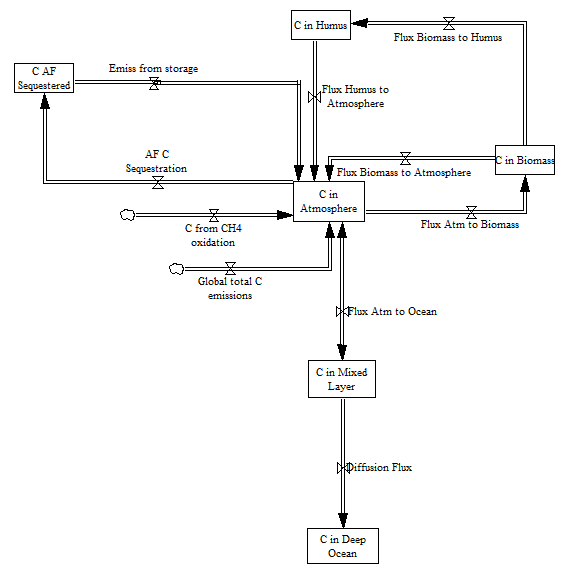
\includegraphics{c-roads-co2}
\caption{C-ROADS-ilmastomallin yksinkertaistettu alimalli hiilidioksidille. \label{ilmasto:co2}}
\end{figure}

Tom Fiddaman mallintaa ilmaston lämpenemistä systeemidynaamisesti jakaen mallin kahteen osaan: hiilidioksidi- ja lämpövarastoihin. 

\subsection{En-ROADS-ilmastomalli \label{ilmasto:enroads}}

\subsection{Muita ilmastomalleja \label{ilmasto:muut}}


\clearpage

%\section{Tulokset}
%\section{Results}


%\clearpage

\section{Yhteenveto \label{yhteenveto}}
%\section{Summary} 

\clearpage

\phantomsection
\addcontentsline{toc}{section}{Viitteet}
\bibliographystyle{plain}
\bibliography{viitteet}

\end{onehalfspacing} % KYPSYYSNÄYTETTÄ VARTEN


\end{document}

